\documentclass[a4paper, 11pt]{beamer}
\usepackage[utf8]{inputenc}
\usepackage[ngerman]{babel}

\usepackage{amsmath}
\usepackage{amssymb}
\usepackage{mathtools}

\usepackage{graphicx}
\usepackage[export]{adjustbox}

\usetheme{CambridgeUS}
\usecolortheme{rose}

\title{PPI Präsentation: Kettennäherung}
\author{Johannes Hübers, Cedric Brügmann, PPI11}
\date{23. Januar 2020}

\begin{document}


\begin{frame}
    \maketitle
\end{frame}

\begin{frame}
    \tableofcontents
\end{frame}



\section{Problemstellung}

\begin{frame}
    \frametitle{Problemstellung}

    Anhand von an einer Kette gemessenen Punkten soll die Gestalt der Kette möglichst gut durch
    $$y = ae^{dx} + be^{-dx} + c, \quad a,b,c,d\in\mathbb{R},$$
    beschrieben werden.

    \begin{figure}
        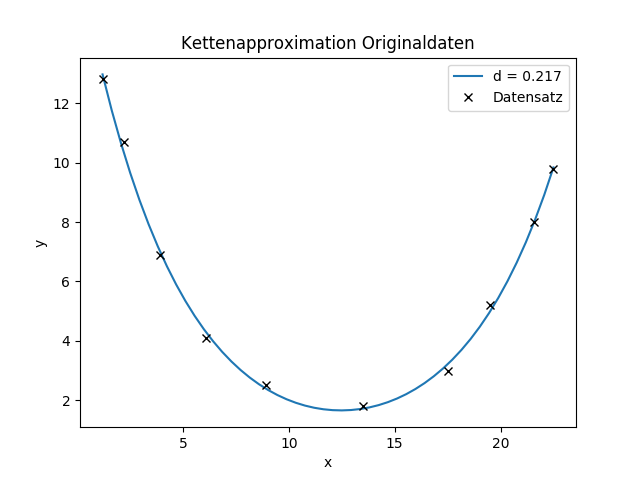
\includegraphics[scale=0.40]{kettenapproximation_originaldaten}
    \end{figure}
\end{frame}



\section{Theorie}

\newcommand{\R}{\left( \begin{array}{c} \hat{R}\\ 0 \end{array} \right)}


\begin{frame}
    \frametitle{QR-Zerlegung}
    Für eine Matrix $A \in \mathbb{R}^{m \times n}, m \geq n$ gibt es eine orthogonale Matrix $Q \in \mathbb{R}^{m \times m}$ und eine obere Dreiecksmatrix $\hat{R} \in \mathbb{R}^{m \times n},$ sodass für
    $$ R \coloneqq \R \text{ gilt, dass } Q \cdot R = A. $$

    Da $A$ überbestimmt ist, gibt es für $Ax = b$ nicht immer eine Lösung in $\mathbb{R}^n.$\\
    \vspace{0.40cm}
    \centering{
    $\Rightarrow$ man sucht nach $x \in \mathbb{R}^n$ mit $\| Ax-b \|_2$ minimal \\
    \vspace{0.1cm}
    $\Leftrightarrow$ $\| Ax-b \|_2^2$ minimal $\Rightarrow x$ heißt Kleinste-Quadrate-Lösung 
}
\end{frame}

\begin{frame}
    \frametitle{Finden der Kleinste-Quadrate-Lösung}

    Für die $QR$-Zerlegung von $A$ ist nun $\| Ax-b \|_2$ minimal genau dann, wenn x nach folgendem Algorithmus berechnet wird:

    \begin{enumerate}
        \item bestimme $z \coloneqq Q^T b,\ z = \left( \begin{array}{r} z_1 \\ z_2 \end{array} \right), \quad z_1 \in \mathbb{R}^n,\ z_2 \in \mathbb{R}^{m-n}$
        \item löse durch Rückwärtseinsetzen das Gleichungssystem $\hat{R}x = z_1$
    \end{enumerate}

    \newcommand{\zo}{\left( \begin{array}{c} z_1\\0 \end{array} \right)}
    \newcommand{\zO}{\left( \begin{array}{c} 0\\z_2 \end{array} \right)}

    Dann ist \begin{alignat*}{2}
        \| Ax-b \|_2 &= \| Q\R x-b \|_2 &&= \| Q \zo - b\|_2 \\
        &= \| Q \zo - Q z \|_2 &&= \| Q \zO \|_2 = \| z_2 \|_2
    \end{alignat*}
    
\end{frame}

\begin{frame}
    \frametitle{Normalengleichung}

    Für $x \in \mathbb{R}^n$ ist $\|Ax-b\|_2$ genau dann minimal, wenn $x$ die Normalengleichung
    $$A^T A x = A^T b \quad \text{löst.}$$
    Ist $A$ vollen Spaltenrangs, ist $A^T A$ invertierbar, also die Kleinste-Quadrate-Lösung eindeutig.

    \vspace{0.25cm}

    Besonders für schlecht konditionierte Matrizen ist aber der $QR$-Algorithmus besser, weil
    $$ cond_2(A) = cond_2(Q^T A) = cond_2(R), $$
    $$ cond_2(A^T A) = cond_2^2(A).$$

\end{frame}




\section{Implementierung}
\newcommand{\x}{\left( \begin{array}{c} x_1\\ \vdots \\x_m \end{array} \right)}
\newcommand{\y}{\left( \begin{array}{c} y_1\\ \vdots \\y_m \end{array} \right)}
\newcommand{\A}{\left( \begin{array}{ccc} e^{dx_1} & e^{-dx_1} & c \\
    &\vdots \\
    e^{dx_m} & e^{-dx_m} & c \end{array} \right)}
\newcommand{\abc}{\left( \begin{array}{c} a \\ b \\ c \end{array} \right)}

\begin{frame}
    \frametitle{Implementierung: Lineares Gleichungssystem für $a,b,c$}

    Für Punkte $(x_k,y_k)$ in der Datenreihe $(x_1, y_1), \hdots, (x_m, y_m)$ soll
    $$ ae^{dx_k} + be^{-dx_k} +c = y_k. $$
    
    Dies ist für feste $d$ äquivalent zur Bedingung
    $$ A(d) \abc = \y, \quad \text{für } A(d) \coloneqq \A \in \mathbb{R}^{m \times 3}$$

    \vspace{\baselineskip}
    Parameter $d$ kann so nicht berechnet werden.

\end{frame}


\begin{frame}
    \frametitle{Implementierung: Lineares Gleichungssystem für $a,b,c$}

    \begin{itemize}
        \item Damit die Kleinste-Quadrate-Lösung von $A(d) \abc = b$ mit der $QR$-Zerlegung für alle $b \in \mathbb{R}^m$ gefunden werden kann, braucht $A$ vollen Spaltenrang
        \item $Q$ ist orthogonal, also invertierbar $\Rightarrow$ reicht Spaltenrang von $R$ zu prüfen: Hat $\hat{R}$ keine Nullen auf der Hauptdiagonalen?
    \end{itemize}
    \vspace{0.2cm}
    \begin{itemize}
        \item Verfahren liefert nur gute Lösungen $a, b, c,$ wenn $d$ zuvor passend gewählt wird
    \end{itemize}
\end{frame}


\begin{frame}
    \frametitle{Implementierung: $d$ ermitteln}

    \begin{itemize}
        \item Verfahren liefert nur gute Lösungen $a,b,c,$ wenn $d$ zuvor passend gewählt wird
    \end{itemize}
    \vspace{0.2cm}
    \begin{itemize}
        \item Dazu einfach im Intervall $[0.1,0.5]$ in gleichen Abständen Werte für $d$ auswählen, $a(d),b(d),c(d)$ berechnen und Normen der Residuen, $\|A\abc-b\|_2$ vergleichen
        \item $d$ mit geringster Residuumsnorm wählen
    \end{itemize}

\end{frame}


\section{Experimente}

\begin{frame}
    \frametitle{Experimente}

    \begin{itemize}
        \item 3 Datensätze: Originaldaten, Datenreihe 2, Datenreihe 3
        \item Bei Datenreihe 2 wurden x- und y-Werte der Datenpaare je auf die nächste ganze Zahl gerundet.
        \item Bei Datenreihe 3 wurden x- und y-Werte der Datenpaare jeweils abgerundet.
    \end{itemize}
    \vspace{0.25cm}
    Fragen:
    \begin{itemize}
        \item Wie wirkt sich $d$ auf die Gestalt der Kettennäherung aus?
        \item Was beeinflusst die Konditionen von $A$ und $A^T A$?
        \item Was beeinflusst die Residuumsnorm?
    \end{itemize}
\end{frame}

\begin{frame}
    \frametitle{Datensätze}

    \begin{figure}
        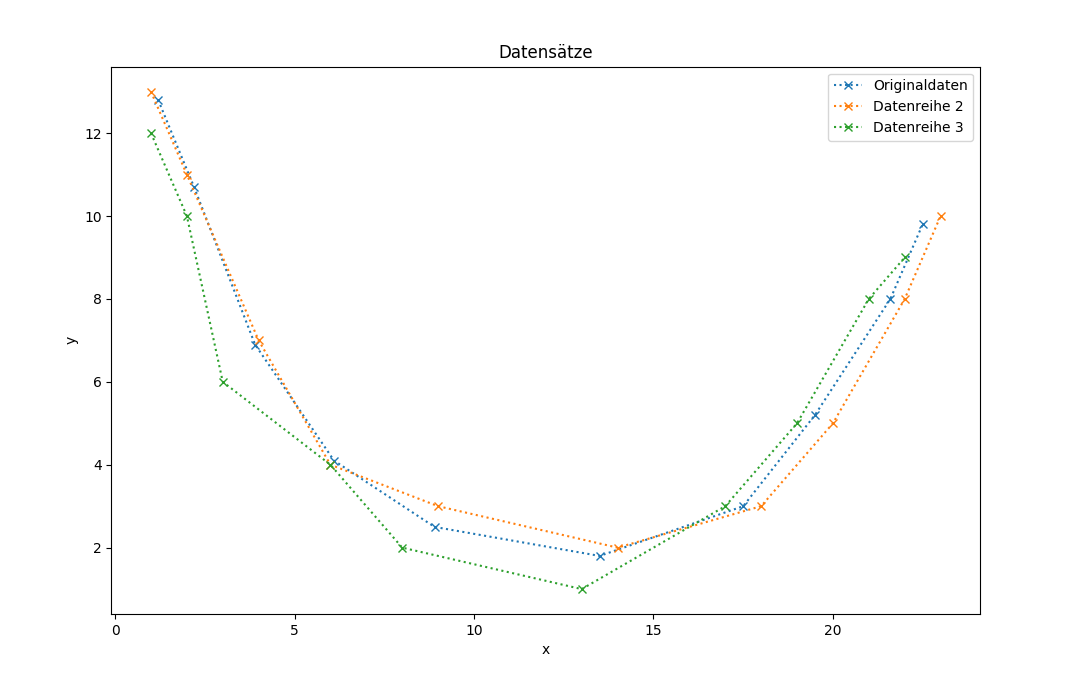
\includegraphics[scale=0.4]{datensaetze}
    \end{figure}
\end{frame}


\begin{frame}
    \frametitle{Kettenapproximationen}

    \begin{figure}
        \centering
        \begin{minipage}{.4\textwidth}
            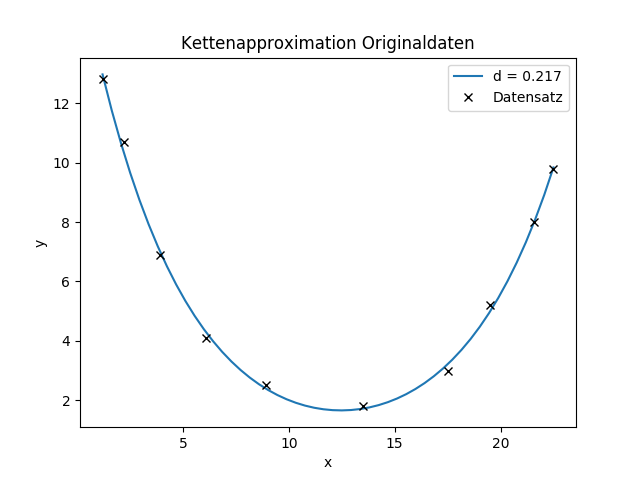
\includegraphics[scale=0.31]{kettenapproximation_originaldaten}
        \end{minipage}
        \begin{minipage}{.4\textwidth}
            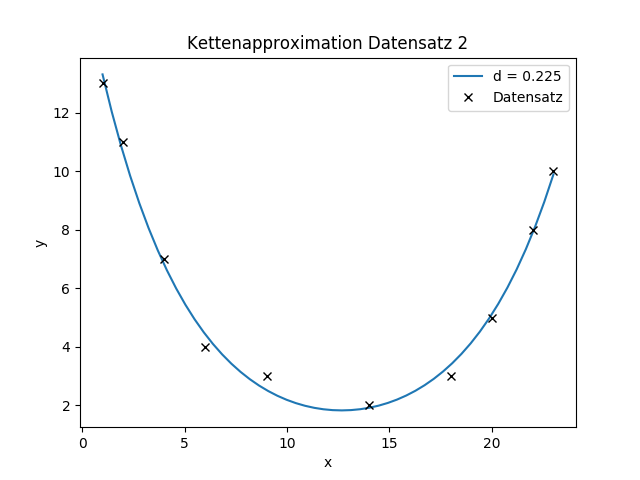
\includegraphics[scale=0.31]{kettenapproximation_ds2}
        \end{minipage}
        \begin{minipage}{.4\textwidth}
            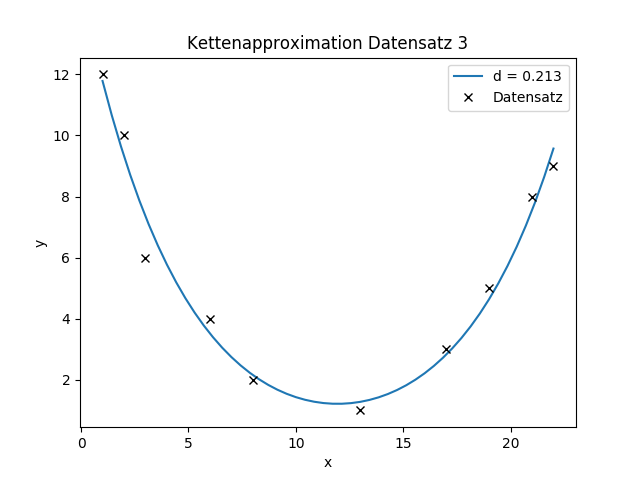
\includegraphics[scale=0.31]{kettenapproximation_ds3}
        \end{minipage}
    \end{figure}
\end{frame}


\begin{frame}
    \frametitle{Approximationen für verschiedene $d$}

    \only<1>{
        \begin{figure}
            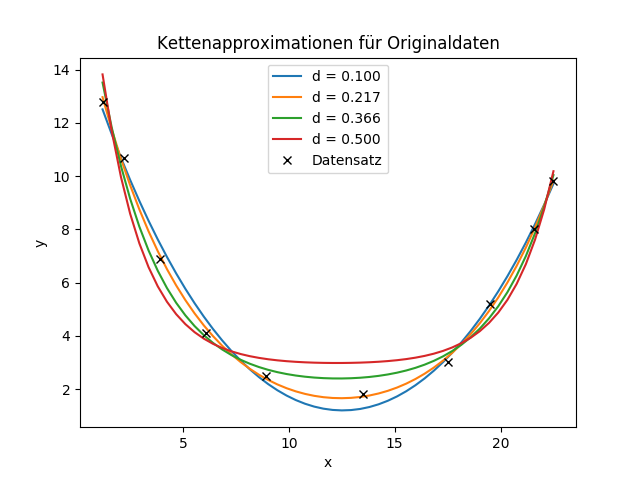
\includegraphics[scale=0.6]{kettenapproximationen_originaldaten}
        \end{figure}
    }

    \only<2>{
        \begin{figure}
            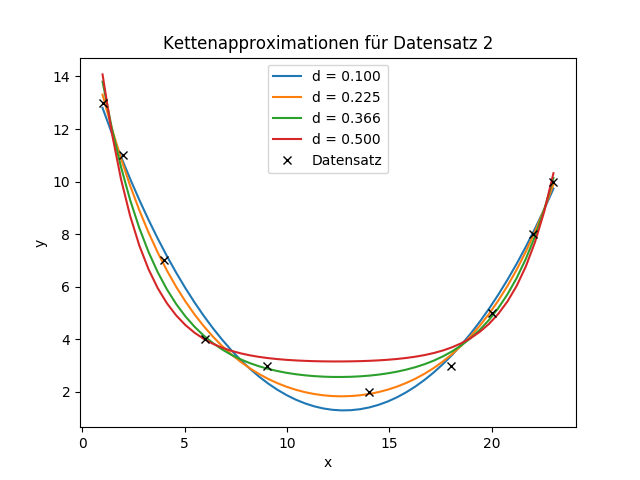
\includegraphics[scale=0.6]{kettenapproximationen_ds2}
        \end{figure}
    }

    \only<3>{
        \begin{figure}
            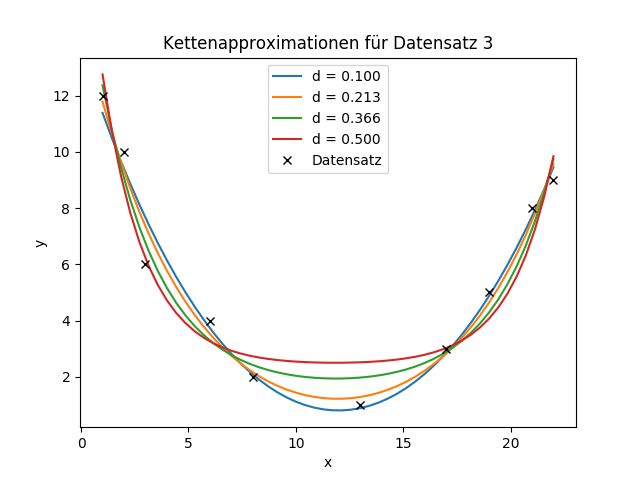
\includegraphics[scale=0.6]{kettenapproximationen_ds3}
        \end{figure}
    }
\end{frame}


\begin{frame}
    \frametitle{Konditionen}

    \begin{figure}
        \centering
        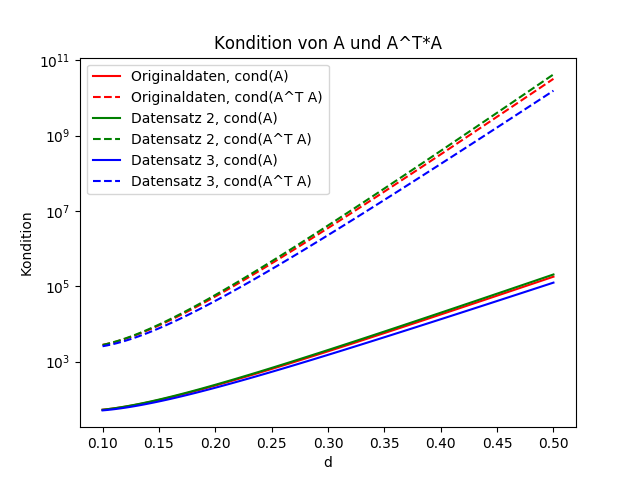
\includegraphics[scale=0.6]{kondition}
    \end{figure}
\end{frame}


\begin{frame}
    \frametitle{Norm des Residuums}

    \begin{figure}
        \centering
        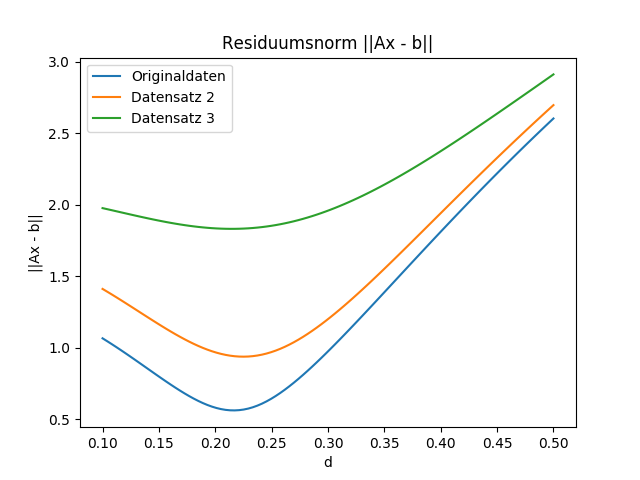
\includegraphics[scale=0.6]{residuumsnorm}
    \end{figure}
\end{frame}


\begin{frame}
    \frametitle{Auswertung}

    \begin{itemize}
        \item Konditionen hängen nur von Werten $x_1,\hdots,x_m$ ab.
        \item Konditionen steigen exponentiell mit d.
        \item Je weniger natürlich die Gestalt des Seils (der Datenreihe), desto höher die Norm des Residuums.
    \end{itemize}
\end{frame}


\section{Literatur}

\begin{frame}
    \frametitle{Literatur}

    \begin{thebibliography}{2}
        \bibitem{NLA}
            Prof. Caren Tischendorf.\\
            \textcolor{black}{Skript Numerische Lineare Algebra, WiSe 2019/20.}
        \bibitem{Blatt}
            Dr. Hella Rabus.\\
            \textcolor{black}{Projektpraktikum I Aufgabenblatt Serie 4, WiSe 2019/20.}
    \end{thebibliography}
\end{frame}

\end{document}
